%
%	Theorieteil
%

\pagebreak
\section{Data Exploration}

\onehalfspacing

\subsection{Access}

Now that we have all the data from wp-statistics in our BigQuery tables, we're ready to start the exploration. 

Let's start by looking at the number of visitors this year. We can see a huge spike around the global climate strike on March 19 and a smaller one before Easter:

\begin{figure}[H]
\centering
\caption {Visitors 2021}
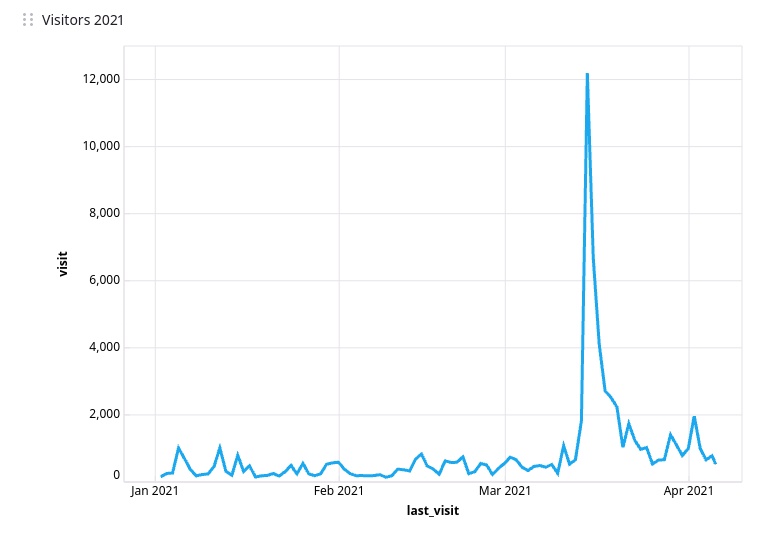
\includegraphics[width=\linewidth]{images/figure01.png}
\label{fig:visitors2021}
\end{figure}

A global climate strike is a significant event in our groups' calendar, and I am pretty happy that we were able to provide our readers with sufficient information about it.

Let's move to the past year. We can see similar significant spikes around the dates for global and local strikes, and local elections:

\begin{figure}[H]
\centering
\caption {Visitors 2020}
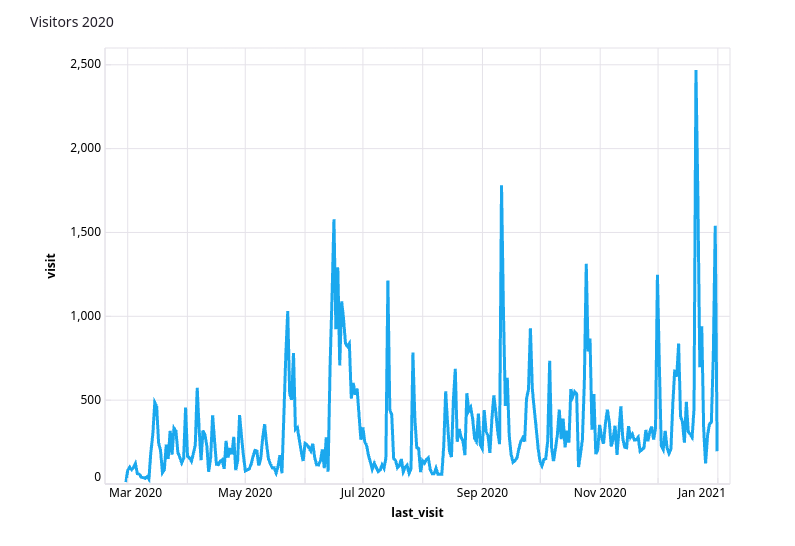
\includegraphics[width=\linewidth]{images/figure02.png}
\label{fig:vistors2020}
\end{figure}

The external calendar data again correlates with the access data; the blog thus seems to fulfill an essential role in keeping our community informed and engaged.

\subsection{Search Engines}

In addition to the people who have bookmarks for the blog, a significant amount of traffic comes from the major search engines:

\begin{figure}[H]
\centering
\caption {Search Engines}
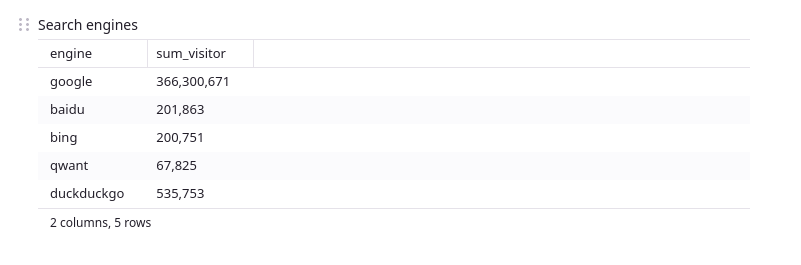
\includegraphics[width=\linewidth]{images/figure03.png}
\label{fig:searchEngines}
\end{figure}

Google is the market leader, but DuckDuckGo is a (distant) runner-up, and we'll see DuckDuckGo again a little bit further down.

Looking at the main key words, we find "Klimastreik" (climate strike) and "Wahl" (local elections) in various forms in our data:

\begin{figure}[H]
\centering
\caption {Search Term Streik}
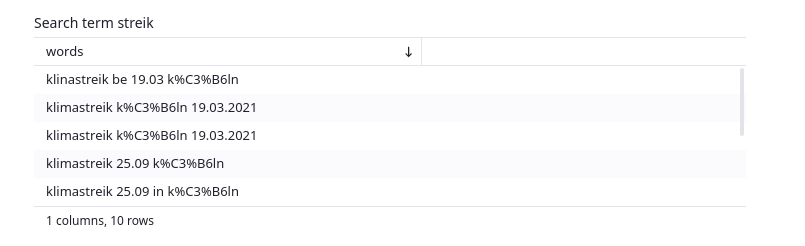
\includegraphics[width=\linewidth]{images/figure04.png}
\label{fig:searchStreik}
\end{figure}

\begin{figure}[H]
\centering
\caption {Search Term Wahl}
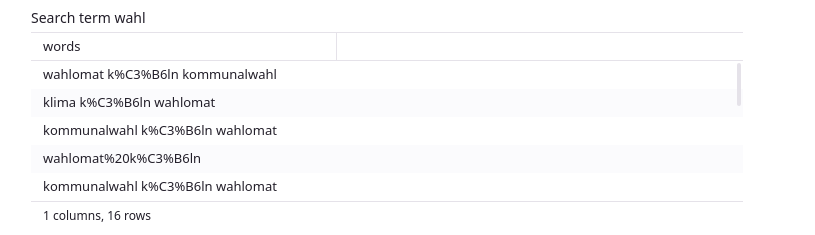
\includegraphics[width=\linewidth]{images/figure05.png}
\label{fig:searchWahl}
\end{figure}

This data supports our findings so far that people inside and outside the community turn to the blog for information for the regular climate strikes and the local elections.

\subsection{Admin Access}

Because we have the data, let's have a look where our admin users come from:

\begin{figure}[H]
\centering
\caption {Admin Access}
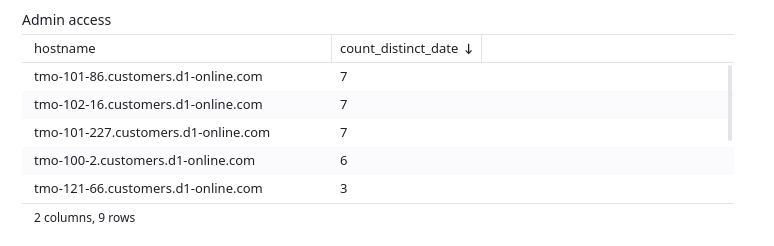
\includegraphics[width=\linewidth]{images/figure06.png}
\label{fig:adminAccess}
\end{figure}

Not surprisingly, with a few exceptions, admin access seems to come from the Deutsche Telekom network, the primary carrier in Germany. Not that this data point is of huge interest, but we can at least rest assured that we most likely were not hacked or pwned.

\subsection{Referrals}

A much more interesting data point than admin access is the referrals, this time not from the wp-search index but from the wp-visitor table itself:

\begin{figure}[H]
\centering
\caption {Referrals}
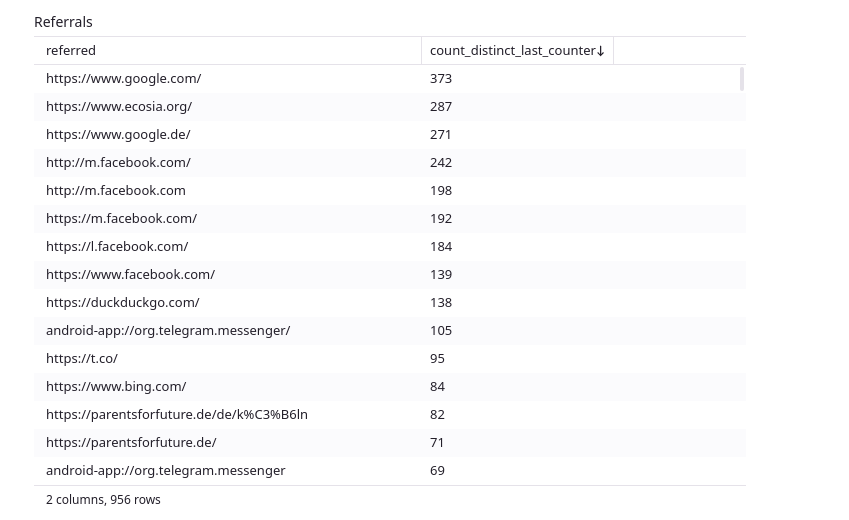
\includegraphics[width=\linewidth]{images/figure07.png}
\label{fig:referrals}
\end{figure}

We can still see Google and other major search engines in the referrals. Still, interestingly enough, the more privacy-oriented ones (\href{https://www.ecosia.org/?c=en}{Ecosia}, \href{https://duckduckgo.com/}{DuckDuckGo}) are pretty high on the list. 

In addition, we can also see several referrals from our Twitter, Facebook, and Telegram channels. It indicates a solid connection with the community and tight integration of the blog with our other social media sources, which is the blog's primary goal.

To keep the community together, to combat loneliness and climate anxiety, a strong connection through as many virtual channels as possible is vital for our outreach work.

\subsection{Platforms}

As we previously saw in the referrals, the number of people in our community using alternative search engines is relatively high. Will we see the same differences when we look at the OS and browser?

Let's start with the operating system:

\begin{figure}[H]
\centering
\caption {Operating System}
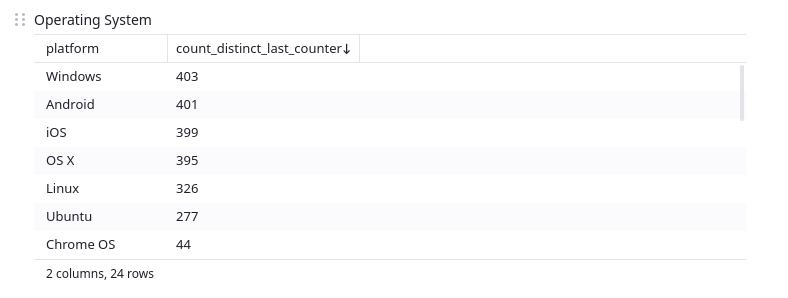
\includegraphics[width=\linewidth]{images/figure08.png}
\label{fig:operatingSystem}
\end{figure}

Access from mobile is pretty evenly split between Android and iOS, as I would expect it to be. 

However, the desktop distribution looks quite interesting: Even though Windows and Mac OS X are again pretty tight, the number of Linux users is far higher once we sum up all the distributions. It is a very different distribution from the overall distribution of desktop operating systems, where the percentage of Linux users usually is in the lower single digits.\footnote{See \textit{Frank, C. (2021)}: Web Traffic Analysis - Predicting Blog Post Performance. \cite{previousBigData}}

Now, let's look at the browser figures:

\begin{figure}[H]
\centering
\caption {Browser}
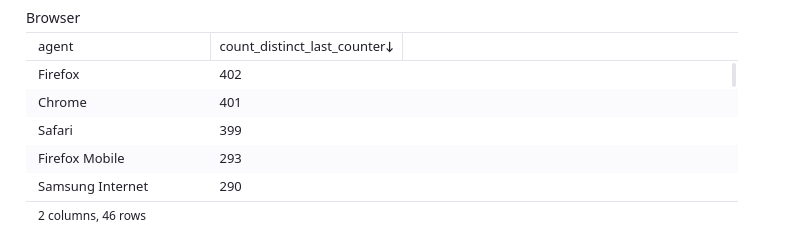
\includegraphics[width=\linewidth]{images/figure09.png}
\label{fig:browser}
\end{figure}

Again, this is a very different and exciting distribution: Firefox and Firefox Mobile together are leading the access, easily outperforming Chrome or Safari. 

This distribution is a continuation of what we saw before. Our community of climate activists does not like to rely on mainstream search engines, mainstream operating systems, or mainstream browsers.

A quick test on \href{https://webpagetest.org/}{WebPageTest} showed a significant difference in loading times and \href{https://web.dev/vitals/}{web vitals} for Chrome and Firefox. Given the high number of Firefox users on our blog, there's room for improvement here.

From the data, there are a couple of key takeaways for the future before we move on to the next chapter:

\begin{itemize}
 \item We should focus SEO more on Ecosia and DuckDuckGo, and less on Google
 \item Firefox is the most prevalent browser, on the Desktop and mobile devices, we should optimize the blog theme for it
 \item Quite surprisingly, Linux is the most favored desktop operating system; we should take that into account for all media formats, especially for images and videos
 \item Mobile access is important, even though still less than 50\%, and we should improve the interface design and speed by optimizing the theme for mobile access
\end{itemize}
